\documentclass[12pt, notitlepage]{article}
\usepackage{amsmath}
\usepackage{amssymb}
\usepackage{amsthm}
\usepackage{listings}
\usepackage{color}
\usepackage{epsfig,graphicx,subfigure}
\usepackage{float}
\usepackage{bm}

\definecolor{dkgreen}{rgb}{0,0.6,0}
\definecolor{gray}{rgb}{0.5,0.5,0.5}
\definecolor{mauve}{rgb}{0.58,0,0.82}

\lstset{
	frame=single,
	language=Java,
	belowskip=3mm,
	showstringspaces=false,
	columns=flexible,
	captionpos=b,
	basicstyle={\small\ttfamily},
	numbers=left,
	numbersep=5pt,
	%numbers=none,
	numberstyle=\tiny\color{gray},
	keywordstyle=\color{blue},
	commentstyle=\color{dkgreen},
	stringstyle=\color{mauve},
	breaklines=true,
	breakatwhitespace=true,
	tabsize=3
}


\providecommand{\abs}[1]{\lvert#1\rvert}
\providecommand{\norm}[1]{\lVert#1\rVert}

\newtheorem{thm}{Theorem}
\newtheorem{lemma}[thm]{Lemma}
\newtheorem{fact}[thm]{Fact}
\newtheorem{cor}[thm]{Corollary}
\newtheorem{eg}{Example}
\newtheorem{ex}{Exercise}
\newtheorem{defi}{Definition}
\newtheorem{hw}{Homework}
\newenvironment{sol}
  {\par\vspace{3mm}\noindent{\it Solution}.}{\qed}

\newcommand{\fib}{\mbox{fib}}
\newcommand{\ov}{\overline}
\newcommand{\cb}{{\cal B}}
\newcommand{\cc}{{\cal C}}
\newcommand{\cd}{{\cal D}}
\newcommand{\ce}{{\cal E}}
\newcommand{\cf}{{\cal F}}
\newcommand{\ch}{{\cal H}}
\newcommand{\cl}{{\cal L}}
\newcommand{\cm}{{\cal M}}
\newcommand{\cp}{{\cal P}}
\newcommand{\cz}{{\cal Z}}
\newcommand{\eps}{\varepsilon}
\newcommand{\ra}{\rightarrow}
\newcommand{\la}{\leftarrow}
\newcommand{\Ra}{\Rightarrow}
\newcommand{\dist}{\mbox{\rm dist}}
\newcommand{\bn}{{\mathbf N}}
\newcommand{\bz}{{\mathbf Z}}

\setlength{\parindent}{0pt}
%\setlength{\parskip}{2ex}
\newenvironment{proofof}[1]{\bigskip\noindent{\itshape #1. }}{\hfill$\Box$\medskip}

\usepackage{enumerate,fullpage, proof}
\newcommand{\Infer}[2]{\infer{#2}{#1}}

\title{Homework 2}
\author{Team: nogg\footnote{E-mail: \texttt{kimi.ysma@gmail.com}}\footnote{Team member: Ma Yesheng, Zhao Ming, Hu Hu, Zou Yikai, Fan Minghua}}

\begin{document}

{\bf\small CS214: Algorithms and Complexity}\hfill{\bf\small 2016 Fall}
{\let\newpage\relax\maketitle}


\begin{ex}\end{ex}
\begin{sol}\\
	\textbf{Observation.1} ~We can find that the array A's size is n and n is even, so  we can divide the array into $\frac{n}{2}$ pairs.\\
	\textbf{Observation.2} ~If we have two arrays, the biggest number among these arrays must be either the first array's biggest number or the second array's biggest number.\\\\
	\emph{step1.} Divide the array into $\frac{n}{2}$ pairs which counts from 1 to $\frac{n}{2}$. \\
	\emph{step2.} Inside each pairs we do one comparison to determine which one is bigger and which one is smaller.\\
	\emph{step3.} Now we get two arrays, one is composed of the bigger one of each pair, another is composed of the smaller one of each pair.\\
	\emph{step4.} Find the biggest number $N_b$ in the first array and the smallest number $N_s$ in the second array.\\
	\emph{step5.} Now the biggest number of A is $N_b$ and smallest number of A is $N_s$. \\\\
	\textbf{Analysis:}In step2 we do $\frac{n}{2}$ comparisons, and in step4 we do ($\frac{n}{2}$-1)+($\frac{n}{2}$-1).Totally, we do $\frac{n}{2}$ + ($\frac{n}{2}$-1) + ($\frac{n}{2}$-1) = $\frac{3n}{2}$-2 comparisons.
\end{sol}


\begin{ex}\end{ex}
\begin{sol}
	\textbf{Observation.}~We have known that we need at least (n-1) times comparisons to find the biggest numbers.\\
	
	\emph{step1.} We find the biggest number in the array through Dividing and Comparing. That is to say, assuming we have a full binary tree which has $2^k$ leaf nodes, and every leaf store a number of the array, and the inside node stores a value which is the bigger one of his sons.\\
	So we have to do $(2^{k-1}+2^{k-2}+...+1)$ = $(2^k-1)$ comparisons to find the biggest one. i.e (n-1) comparisons.\\
	
	\textbf{Observation.} The second-biggest number in the array must have done comparison with the biggest one during the construction of the full binary tree.\\
	\textbf{Proving.} Assuming the biggest number is $N_1$, and the second-biggest number is $N_2$. If $N_2$ hasn't compared with $N_1$, it must be smaller that a number, and that number is not $N_1$, so $N_2$ is at least third-biggest number, which is not same with the assumption.\\
	
	\emph{step2.} Get the numbers which have compare with $N_1$, there will be $log_2(n)$, which is the height of the full binary tree. Find the biggest number of these $log_2(n)$ numbers.\\
	
	\textbf{Analysis:}~In step1. we do (n-1) comparisons, and in step2. we do ($log_2(n)$-1) comparisons. Totally, we do (n + $log_2(n)$ - 2) comparisons.
\end{sol}


\begin{ex}\end{ex}
\begin{sol}
	\textbf{Analysis:}~Given an array A which contains 3 elements $a_1,a_2,a_3$, and these 3 elements is different from each other. According to the given algorithm, we only need one comparison to find the largest number. However, we can compare two elements one time. And no matter how we choose the elements, there is still one element will not be compared and we cannot know whether it is bigger or smaller. So the algorithm is absolutely wrong.
\end{sol}


\begin{ex}\end{ex}
\begin{sol}
	
\end{sol}


\begin{ex}\end{ex}
\begin{sol}
	
\end{sol}


\begin{ex}\end{ex}
\begin{sol}\\ \\
	In quicksort, we use a pivot number randomly chosen to divide the number sequence ito two part. Then we need to do the same quicksort operation on each part and repeat it. But in quickselect, similarly, in each recursion step, we need to divide the sequence into two part, but we only need to do the same quickselect operation on one of them. Which means that, in quickselect, we only need to do "partial execution" in each step of quicksort. Therefore, quickselectcan be viewed as a "partial execution" of quicksort. \\ \\
	We use the sequence \{4, 7, 9, 3, 1, 2, 6, 5, 8\} as an example. The quicksort tree is drawn above.\\
	In order to select the $5th$ number in this sequence, the part in red circle is visited by quickselect.
	\begin{figure}[H]
		\center
		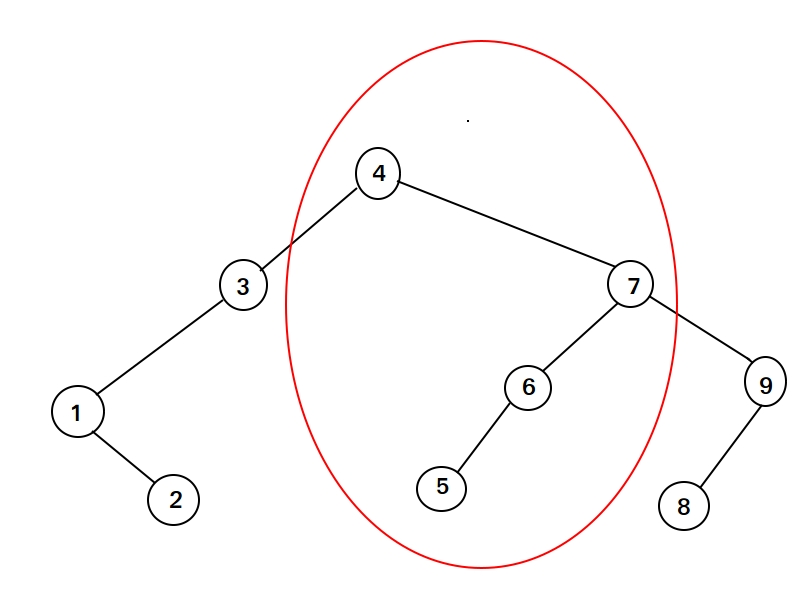
\includegraphics[width=0.8\linewidth]{p1.jpg}\vspace{-10pt}
		\caption{quicksort tree of [4, 7, 9, 3, 1, 2, 6, 5, 8]} \nonumber\label{fig:quicksort tree}\vspace{-10pt}
	\end{figure}

\end{sol}


\begin{ex}\end{ex}
\begin{sol}\\ \\
	Obviously,\\
	$\mathbb{E}[B_{i,j,k}]=\bm{P}(B_{i,j,k}=1)$\\
	(Which P(A) means the probability of event A)\\ \\
	Notice that $B_{i,j,k}=A_{i,j}\ \&\&\ A_{i,k}$\\ 
	(Which $A_{i,j}$ is an indicator variable which is 1 if i is an ancestor of j in the tree T(π), and 0 otherwise as same as in lecture)\\ \\
	Then,\\
	$\mathbb{E}[B_{i,j,k}]=\bm{P}(A_{i,j}=1\ \&\&\ A_{i,k}=1)$\\
	=\ $\bm{P}(A_{i,j}=1)*\bm{P}(A_{i,k}=1)$\\
	=\ $\infer{(|i-j|+1)*(|i-k|+1)}{1}$\\
\end{sol}


\begin{ex}\end{ex}
\begin{sol}
	
\end{sol}


\begin{ex}\end{ex}
\begin{sol}
	
\end{sol}

\end{document}
